\section{Implementation and Experiments}

\subsection{Clause Reduction with $\IUIP$}
To evaluate $\IUIP$'s effectiveness as a clause reduction technique, we implement  $\IUIPPURE$ and $\IUIPMIN$  on top of \text{\MapleBase} \cite{}, the winner of SAT Race 2015 application track.  We than compare the performance of the baseline $\MapleBase$ with $\MapleIUIPPURE$ and $\MapleIUIMIN$ on the full set of benchmarks from SAT RACE 2019 main track.

The benchmark contains 400 instances divided into two groups of 200, new and old, representing historical instances and fresh instances in the 2019 race, respectively. I partition the old group instances into six partitions of size 30 and one partition of size 20. Each partition is then assigned to a Intel CPU node with 16 cores (2 sockets 8 cores  and  1 thread) and 96649 MB memory. The new group is partitioned based on their contributor (e.g. Heule contributed 22 matrix multiplication instances), and each partition is assigned to a aforementioned CPU node. To speed up the experiment, we allow a CPU node to solver at most seven instances concurrently. 

Beside solved instances count and PAR-2 score, we additionally measure the average clause length and clause reduction ratio for each instances. For $\MapleIUIPPURE$  and $\MapleIUIMIN$, we also captures the $\IUIP$ learning attempted rate and success rate.

\begin{figure} 
\begin{center}
\begin{tabular}{ | m{3.5cm} | m{2cm}| m{2cm} | m{2cm} | m{2.5cm} | } 
\hline
Solver & \# solved & PAR-2 & Clause Size & Cl Reduction\% \\ 
\hline
$\MapleBase$ & 221 & 5018.89 & 62.6 & 36.53\% \\ 
\hline
$\MapleIUIPPURE$ & 226 & 4920.04 & 49.6 & 41.6\% \\ 
\hline
$\MapleIUIMIN$ & 226 & 4890.67 & 45.2 & 47.8\%\\ 
\hline
\end{tabular}
\end{center}
\caption{Benchmark results of $\MapleBase$ , $\MapleIUIPPURE$  and $\MapleIUIMIN$ on SAT2019 race main track.}
\label{fig:t1}
\end{figure}

Fig.~\ref{fig:t1} shows that both version of $\IUIP$ solved five more instances than the baseline solver with lower PAR-2 scores. $\IUIPMIN$ has marginally lower PAR-2 score than $\IUIPPURE$. Both $\IUIPPURE$ and $\IUIPMIN$ produce clause with significantly smaller size than 1-UIP by 27.7\% and 20.7\%, respectively. Fig.~\ref{fig:len_pdf} shows the probability density distribution (PDF) of the average clause length from $\IUIPMIN$ relative to 1-UIP. $\IUIPMIN$ learning produces shorter clauses for 88.25\% instances, and average relative reduction from 1-UIP is 18.685\%.Fig.~\ref{fig:len_compare} compares the absolute average clause size from $\IUIPMIN$ and 1-UIP, and it shows that $\IUIPMIN$ in general produces smaller clauses, and the size reduction is more significant for instances with large average 1-UIP clause size. 

We also looked at the 14 instances solved by $\IUIPMIN$ but not by 1-UIP. $\IUIPMIN$ produces smaller clauses for all of them with average relative reduction of 22\% and maximum 77\% (30 vs 135). Seven out of 14 instances has size relative reduction over 30\%. For the 9 instances solved by 1-UIP but not by $\IUIPMIN$, $\IUIPMIN$ only produce smaller clause by 33\% and with average relative reduction of 3.3\$.



\begin{figure}
    \centering
    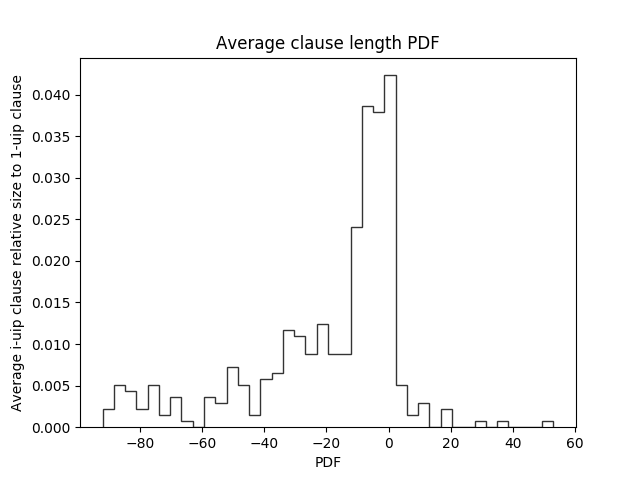
\includegraphics[width=0.8\textwidth,natwidth=610,natheight=642]{clause_length_PDF.png}
    \caption{Average clause (relative to 1-UIP clauses) size distribution. X axis indicates the relative size difference, and Y axis indicates the PDF.}
     \label{fig:len_pdf}
\end{figure}
\begin{figure} \label{fig:len_compare}
    \centering
    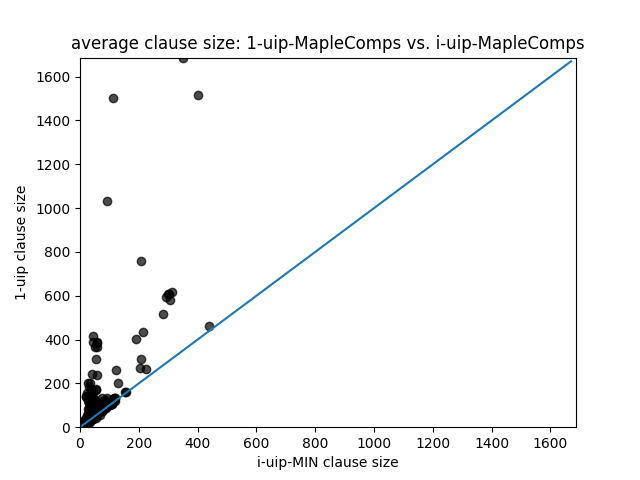
\includegraphics[width=0.8\textwidth,natwidth=610,natheight=642]{i-uip-sizes-compare.png}
    \caption{Average clause size comparison plot. Each point in the plot represents an benchmark instance. X and Y axis shows the clause length from $\MapleIUIMIN$ and $\MapleBase$, respectively  }
    \label{fig:len_compare}
\end{figure}


$\IUIPMIN$ outperformed $\IUIPPURE$ in both PAR-2 score and clause size.  This results agrees with our observation in Fig.~\ref{fig:t2}: $\IUIPMIN$ attempted $\IUIP$ learning more frequently, and it is more likely to succeed. Remark that the success of $\IUIP$ learning is determined by the size of the learned i-UIP clause $\iUIPClause$, and the $\IUIP$ learning frequency is also indirectly controlled by $\IUIP$'s success rate from the previous restart interval. The results indicates  $\IUIPMIN$ shortened $\iUIPClause$'s size through further minimization of $\iUIPClause$ at non-unique implication decision level.



\begin{figure} 
\begin{center} 
\begin{tabular}{ | m{3.5cm} | m{5cm}| m{5cm} | } 
\hline
Solver & $\IUIP$ attempt rate & $\IUIP$ success rate  \\ 
\hline
$\MapleIUIPPURE$ & 16.1\% & 43.4\% \\ 
\hline
$\MapleIUIMIN$ & 28.8\% & 59.3\% \\ 
\hline
\end{tabular}
\end{center}
\caption{Compare $\IUIPPURE$ and $\IUIPMIN$ i-uip attempt rate and success rate. $\IUIPMIN$ scheme attempted $\IUIP$ more frequently, and it is more likely to successfully produce smaller $\iUIPClause$ clause .}
\label{fig:t2}
\end{figure}

A solver produce smaller clauses can construct smaller proofs. For UNSAT instances, we additionally measure their DRUP\cite{} proof checking time as well as the size of the optimized DRUP proof. We used DART-trim \cite{} with 5000 timeout to check and optimize DRUP proofs. 

Fig.~\ref{fig:t3} shows that the optimized proof construct by $\IUIPMIN$ and $\IUIPPURE$ are significantly smaller than 1-UIP proofs. The relative proof size reduction rougly correlates to the average clause size reduction. Fig.~\ref{fig:proof_compare} shows the absolute proof size comparison results. 

\begin{figure} 
\begin{center} 
\begin{tabular}{ | m{3.5cm} | m{5cm}| m{5cm} | } 
\hline
Solver & optimized proof size (MB) & relative reduction size  \\ 
\hline
$\MapleBase$ & 613.9 & 0  \\ 
\hline
$\MapleIUIPPURE$ & 487.2 & 6.90\% \\ 
\hline
$\MapleIUIMIN$ & 413.2 & 17.18\% \\ 
\hline
\end{tabular}
\end{center}
\caption{Optimized UNSAT proof comparison for 1-UIP $\IUIPPURE$ and $\IUIPMIN$. Optimized proof size measures the average absolute proof size in MB, and relative reduction size measures the average relative reduction for all UNSAT instances.}
\label{fig:t3}
\end{figure}

\begin{figure}
    \centering
    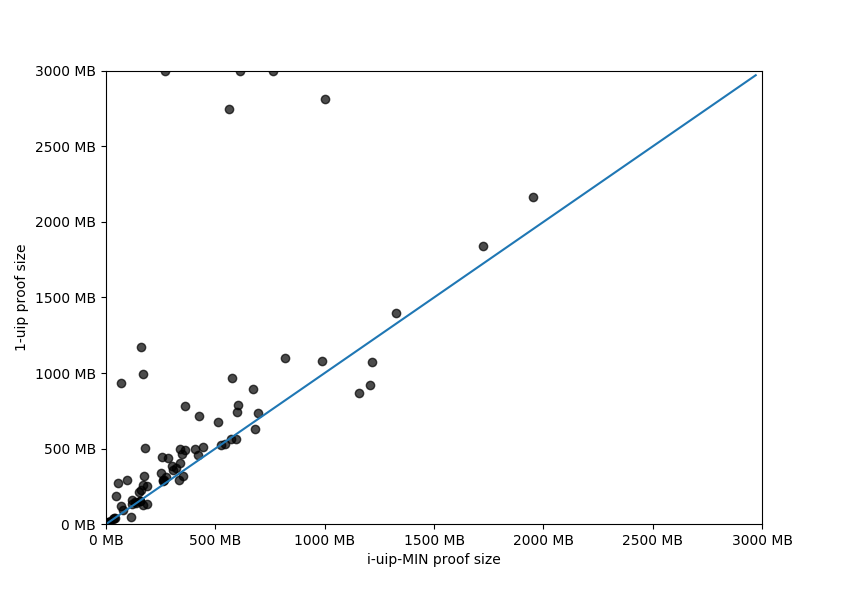
\includegraphics[width=0.8\textwidth,natwidth=610,natheight=642]{proof_size_compare.png}
    \caption{Average optimized proof size between 1-uip and $\IUIPMIN$.}
    \label{fig:proof_compare}
\end{figure}

\subsection{$\IUIP$ as a Practical Learning Scheme}
To evaluate $\IUIP$'s effectiveness as a clause learning scheme, we implement $\IUIPMIN$ on $\MapleBase$ with the extensions mentioned in section~\ref{sec:i-uip}. We evaluated four different configurations (i-UIP, i-UIP-Greedy, i-UIP-Inclusive, and i-UIP-Exclusive) of $\IUIP$ and 1-UIP learning on the SAT Race 2019 main track benchmark and report each configuration's solved instances, PAR-2 score and average clause size. 

Fig.~\ref{fig:t4} summarizes the result of the experiment. Learning scheme i-UIP-greedy solves the same amount of instance (226) as i-UIP with less PAR-2 score. The inclusive activity adjustment solves the most SAT instances (138) and the least UNSAT instances (87). The exclusive activity adjustment scheme produces the shortest average clause size, but solved the second least instances, one more instance than the baseline.  

\begin{figure} 
\begin{center}
\begin{tabular}{ | m{3.5cm} | m{4cm}| m{2cm} | m{2.75cm} |  } 
\hline
Solver & \# solved (SAT, UNSAT) & PAR-2 & Avg clause Size \\ 
\hline
1-UIP & 221 (132, 89)  & 5018.89 & 62.6  \\ 
\hline
i-UIP & \textbf{226} (135, \textbf{91}) & 4890.67 & 45.2 \\ 
\hline
i-UIP-greedy & \textbf{226} (135, \textbf{91})  & \textbf{4866.94} & 47.7 \\
\hline
i-UIP-active-Inclusive & 225 (\textbf{138}, 87) & 4958.49 & 52..12 \\
\hline
i-UIP-active-Exclusive & 223 (134, 89) & 5015.23 & \textbf{43.2} \\
\hline
\end{tabular}
\end{center}
\caption{Benchmark results of 1-UIP ($\MapleBase$), i-UIP($\IUIPMIN$), i-UIP-Greedy,
i-UIP-Inclusive, and i-UIP-Exclusive on SAT2019 race main track.}
\label{fig:t4}
\end{figure}


\nf{Inserted a table here, and graphs and analysis}


\subsection{$\IUIP$ on Modern SAT solvers}
To validate $\IUIP$ as a generalizable learning scheme on modern SAT solvers, we re-implement $\IUIP$ on $\MapleSeven$ \cite{},  $\MapleNine$ \cite{} and $\expSAT$.  
The first two solvers are the winner of 2017 and 2019 SAT race, respectively.  $\expSAT$ is a top ten solver from 2019 SAT race which uses random walk simulation to help branching. For each solver, we compare the base 1-UIP learning scheme against top two $\IUIP$ configurations, $\IUIPGreedy$ and $\IUIPActive$, on the SAT Race 2019 main track benchmark. We report solved instances and PAR-2 score.

\nf{Inserted a table here, and graphs and analysis}
